\chapter{Application implementation}

\section{Backend server}

The backend server does not need to be particularly suited for large traffic or complexity. Its role is only to provide up-to-date GTFS data and manage user accounts. To this end, let's discuss about how it has been implemented.

As mentioned in the previous chapter, I used NestJS with TypeScript to build the backend server. NestJS is an opinionated framework that brings important abstractions (in the form of decorated classes and dependency injection) on top of an already-proven, battle-tested, HTTP server library (Express JS). NestJS can work with plain JavaScript, but augmenting it with TypeScript brings forth is fullest potential.

NestJS is heavily inspired from Angular, thus employs a system of \textit{modules}, that can be loaded into a Nest application individually, along with its dependencies, to the programmer's wish. Organizing into separate modules, or bundling everything into the default App module, is a decision taken by the programmer, taking into consideration applications such as microservices (different modules within the same project can be useful here) and complexity concerns (modules are hard to get to work). I chose to structure my project in modules that correspond to the following functionalities: authentication, GTFS file operation, user management.

\subsection{App module}
\label{sec:AppModule}

The App module is the big module that gets loaded and ran on application bootstrap. Presented in Figure \ref{FigBeBootstrap}, the application bootstrap code will initialize the Nest application using the \verb|AppModule| module as a root module, then takes some final steps in the setup of the environment, by disabling all CORS functionality and allowing all origins, allowing access to static assets (namely, the GTFS data, which is stored locally), and setting up the global \verb|ValidationPipe|, which takes care of request validation. When ready to listen to requests, we take the port from the environment (or use 3000 as default), then we start the Nest application.

\begin{figure}[htbp]
    \centering
    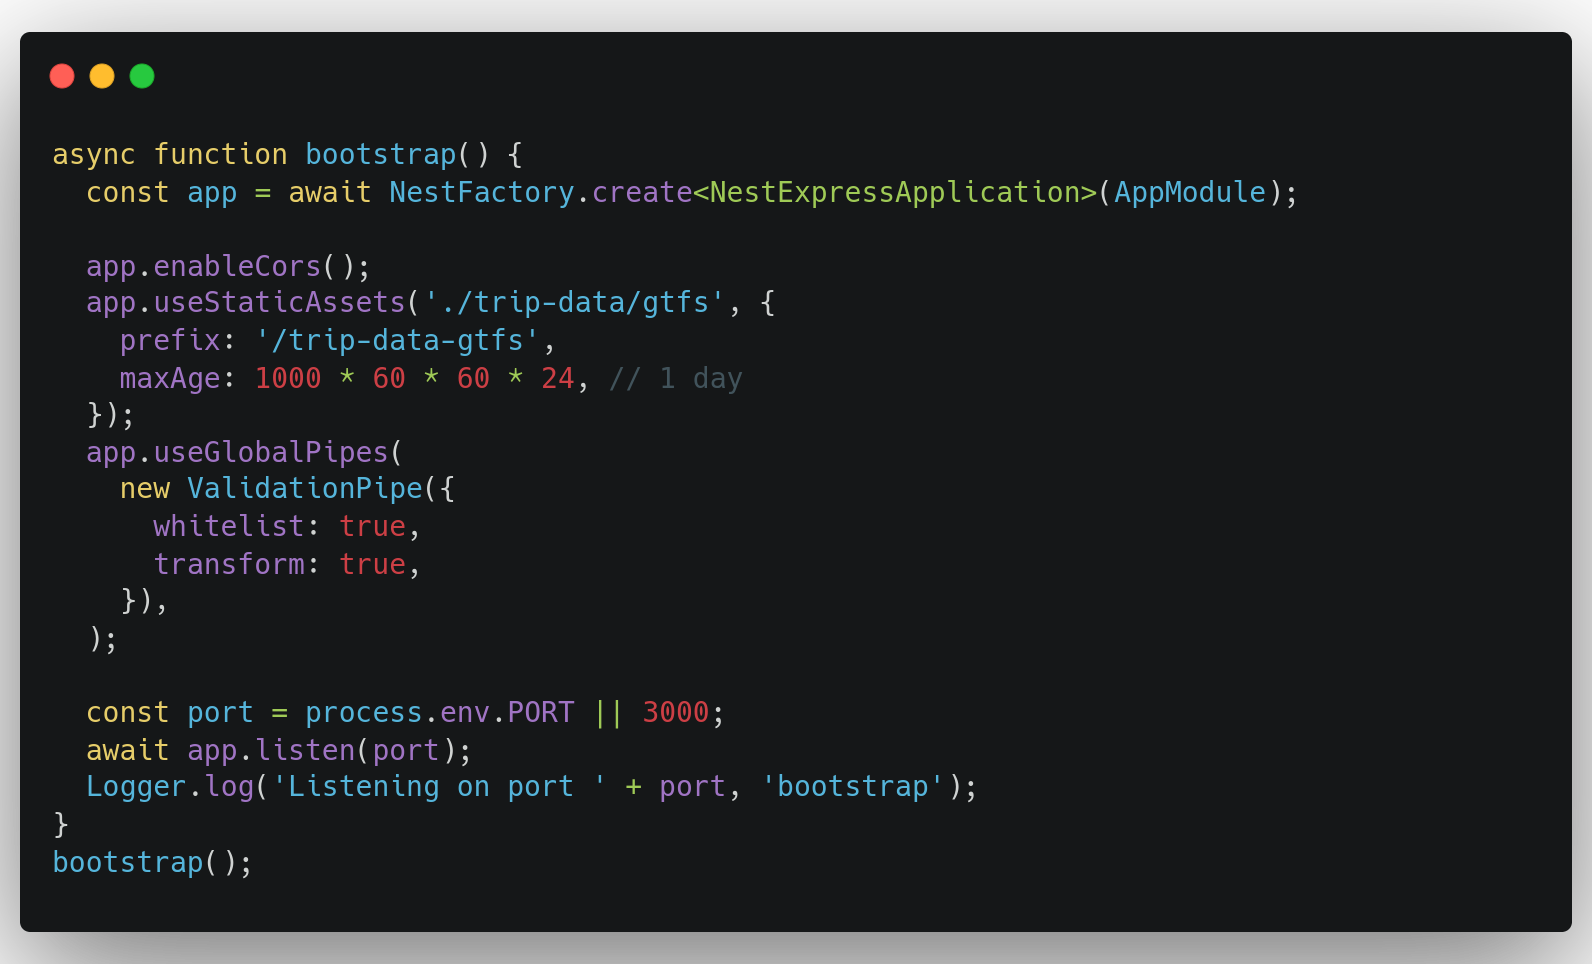
\includegraphics[width=0.9\textwidth]{./figures/code/be_bootstrap.png}
    \caption{Backend: bootstrapping code.}
    \label{FigBeBootstrap}
\end{figure}

Module definitions are not much more complex than importing all the dependency modules and adding them in the module definition, using the \verb|Module| decorator. The definition of the \verb|AppModule| is presented in Figure \ref{FigBeAppModule}, and consists of importing our three modules (auth, GTFS, and user) and the \verb|MongooseModule|, provided by Nest, which offers interaction with MongoDB databases, and the definition of the module class.

\begin{figure}[htbp]
    \centering
    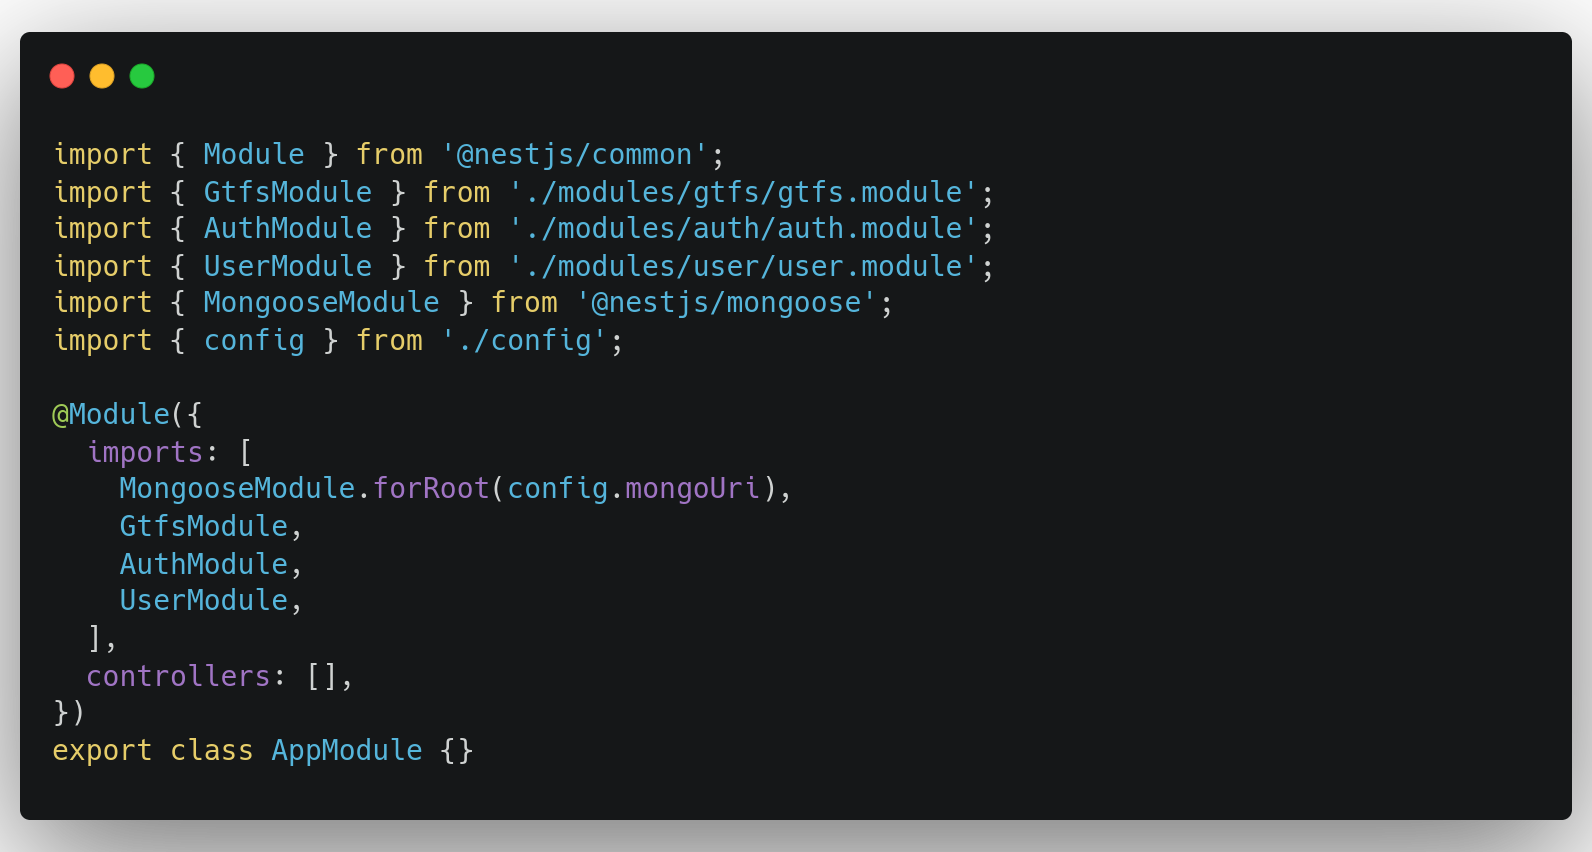
\includegraphics[width=0.9\textwidth]{./figures/code/be_app-module.png}
    \caption{Backend: AppModule.}
    \label{FigBeAppModule}
\end{figure}

\subsection{Configuration}
\label{sec:Configuration}

Backend configuration is stored in a \verb|config.yaml| file at the root of our project. The file is ignored by git, and serves as the location to place all the application secrets and connection instructions, along with configuration that might differ from an environment to the next.

A schema of the configuration file, without actual values, is presented in Figure \ref{FigBeConfig}. We can see configuration related to GTFS (where to download GTFS data from, and what files), along with social authentication secrets, MongoDB database URL, and JWT generation secret.

\begin{figure}[htbp]
    \centering
    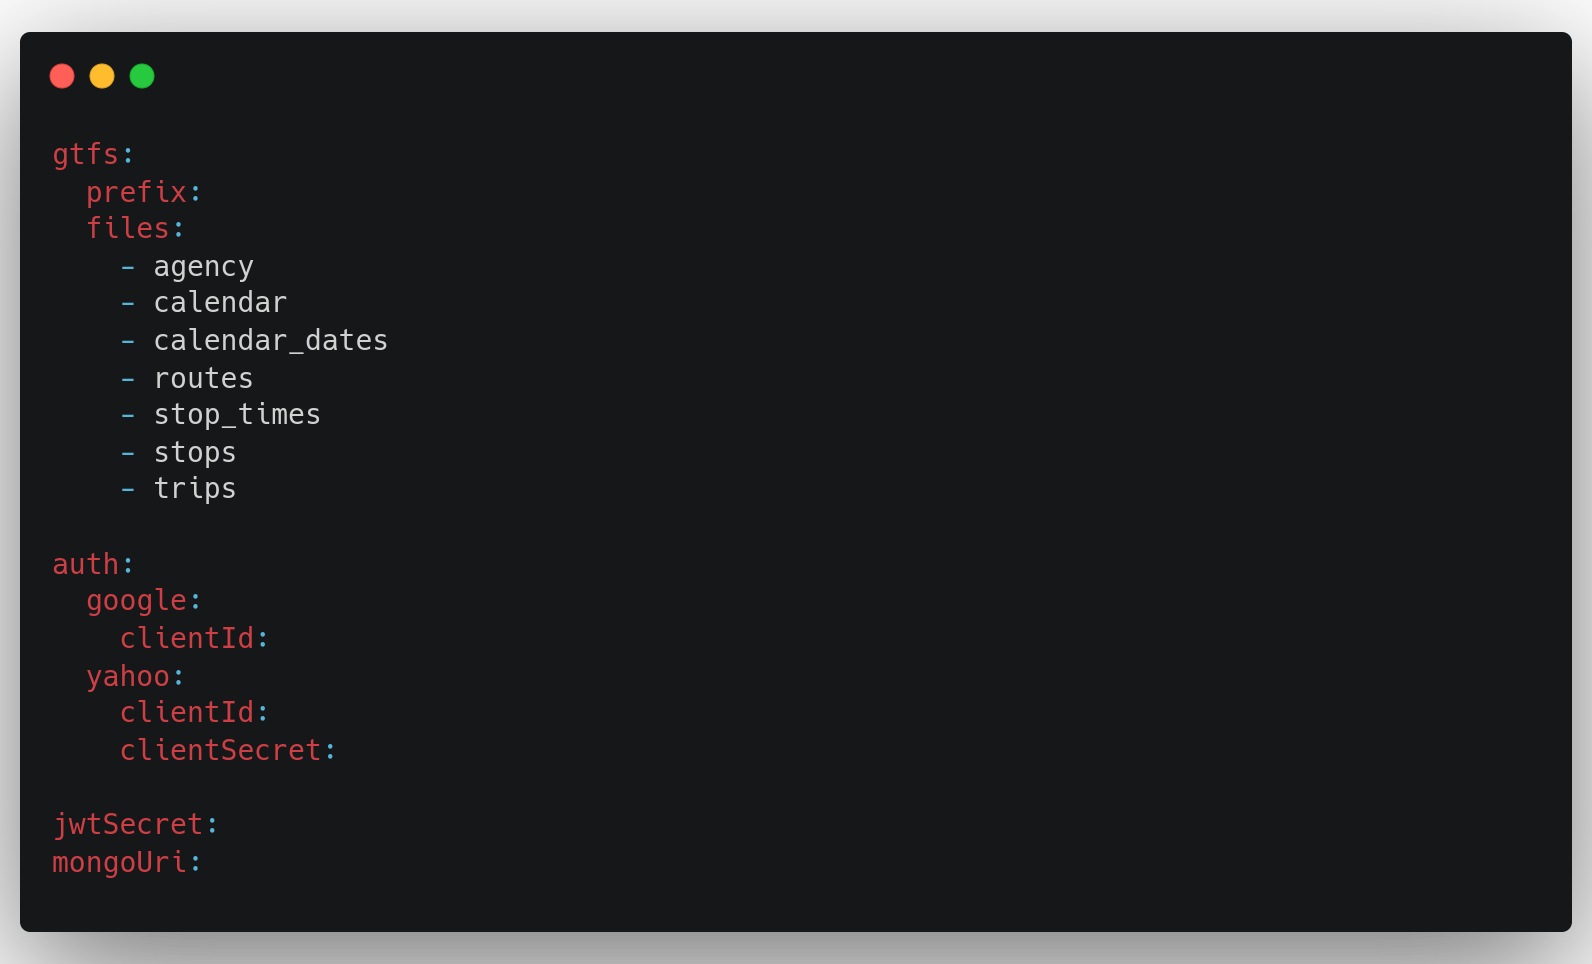
\includegraphics[width=0.9\textwidth]{./figures/code/be_config.png}
    \caption{Backend: config.yaml}
    \label{FigBeConfig}
\end{figure}

The YAML file is then loaded into memory in the \verb|config.ts| TS module, then exported so that it is available for the entire application.

Having the configuration file be loaded by Node is a decision taken in light of simplicity. NestJS offers ways of integrating configuration within its module system, but it requires writing additional code and logic, not only for the providing module, but for modules and services that use the configuration too.

As a safety precaution, the config file is validated against a schema using Joi, which can help identify missing configuration parameters at application startup, rather than have the application crash when it tries to access an inexistent configuration parameter. The Joi schema is presented in Figure \ref{FigBeConfigSchema}.

\begin{figure}[htbp]
    \centering
    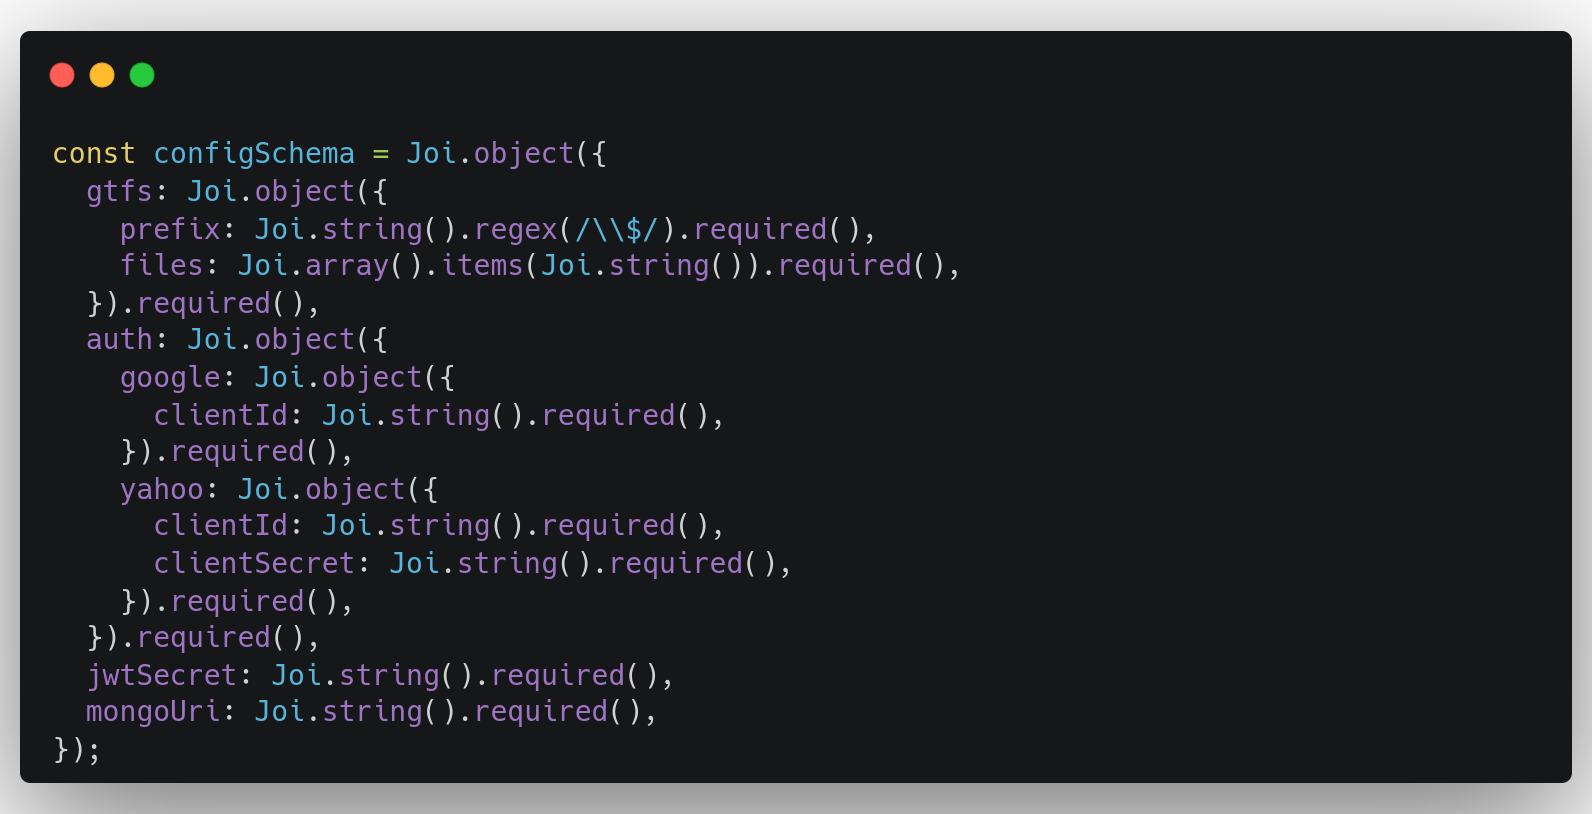
\includegraphics[width=1\textwidth]{./figures/code/be_config-schema.png}
    \caption{Backend: config validation schema.}
    \label{FigBeConfigSchema}
\end{figure}

\subsection{Preparing GTFS data for download}

The GTFS files are available on Vasile Coțovanu's GitHub repository \cite{VasileRubyExporter}, and before serving to our frontend, the files need to be downloaded locally first.

To this end, there exists a script called \verb|process-gtfs.ts|, that when run, creates a Nest application but only loads the GTFS module (Figure \ref{FigBeGTFSBootstrap}). The script then retrieves the \verb|GtfsService| service and uses it to initiate the download of GTFS data from GitHub, which is then placed in the \verb|trip-data| directory. This directory is then referenced in the static assets declaration from the application bootstrapping code (see Section \ref{sec:AppModule}).

\begin{figure}[htbp]
    \centering
    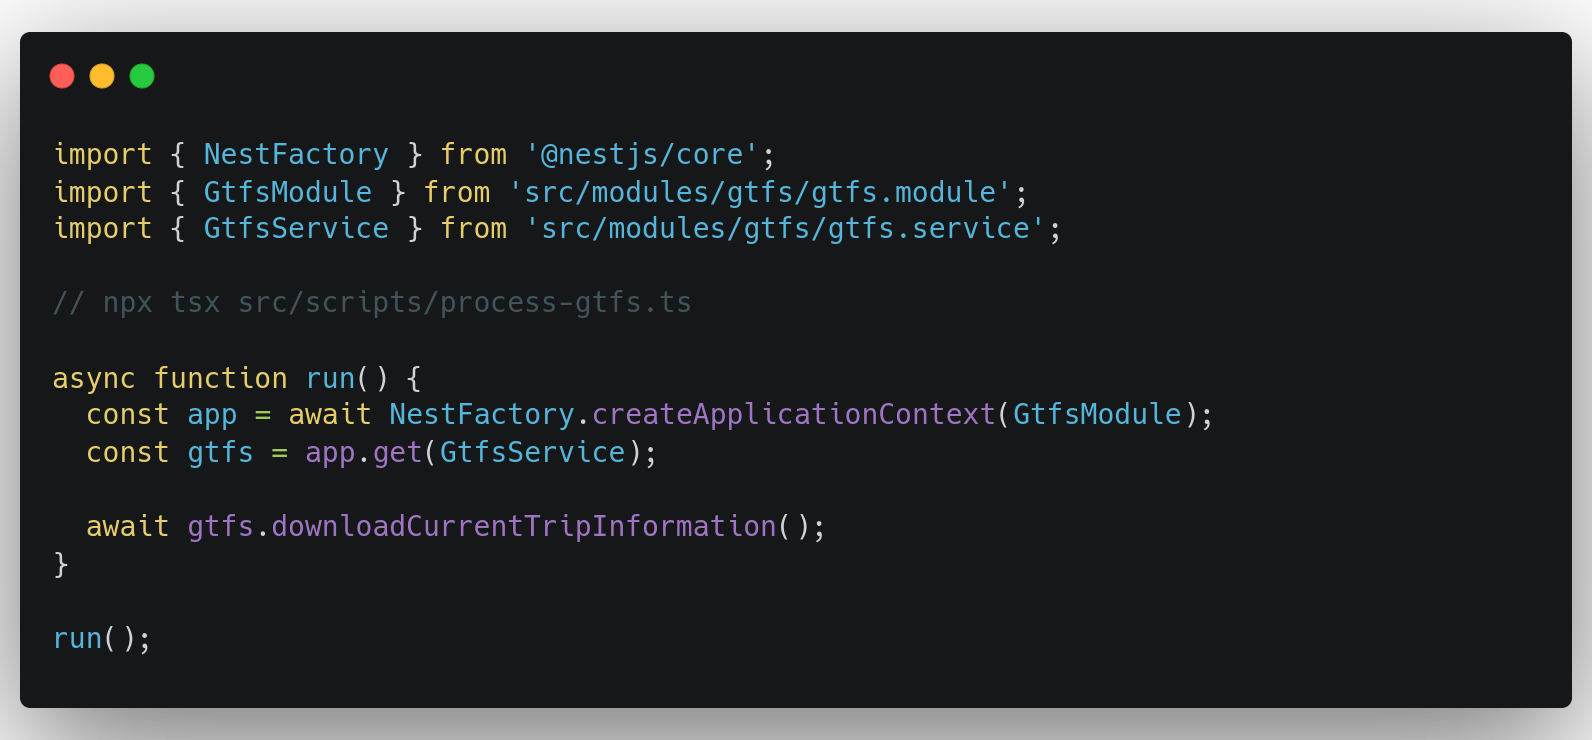
\includegraphics[width=1\textwidth]{./figures/code/be_gtfs-bootstrap.png}
    \caption{Backend: GTFS script bootstrapping code.}
    \label{FigBeGTFSBootstrap}
\end{figure}

\subsection{Auth module}

\begin{figure}[htbp]
    \centering
    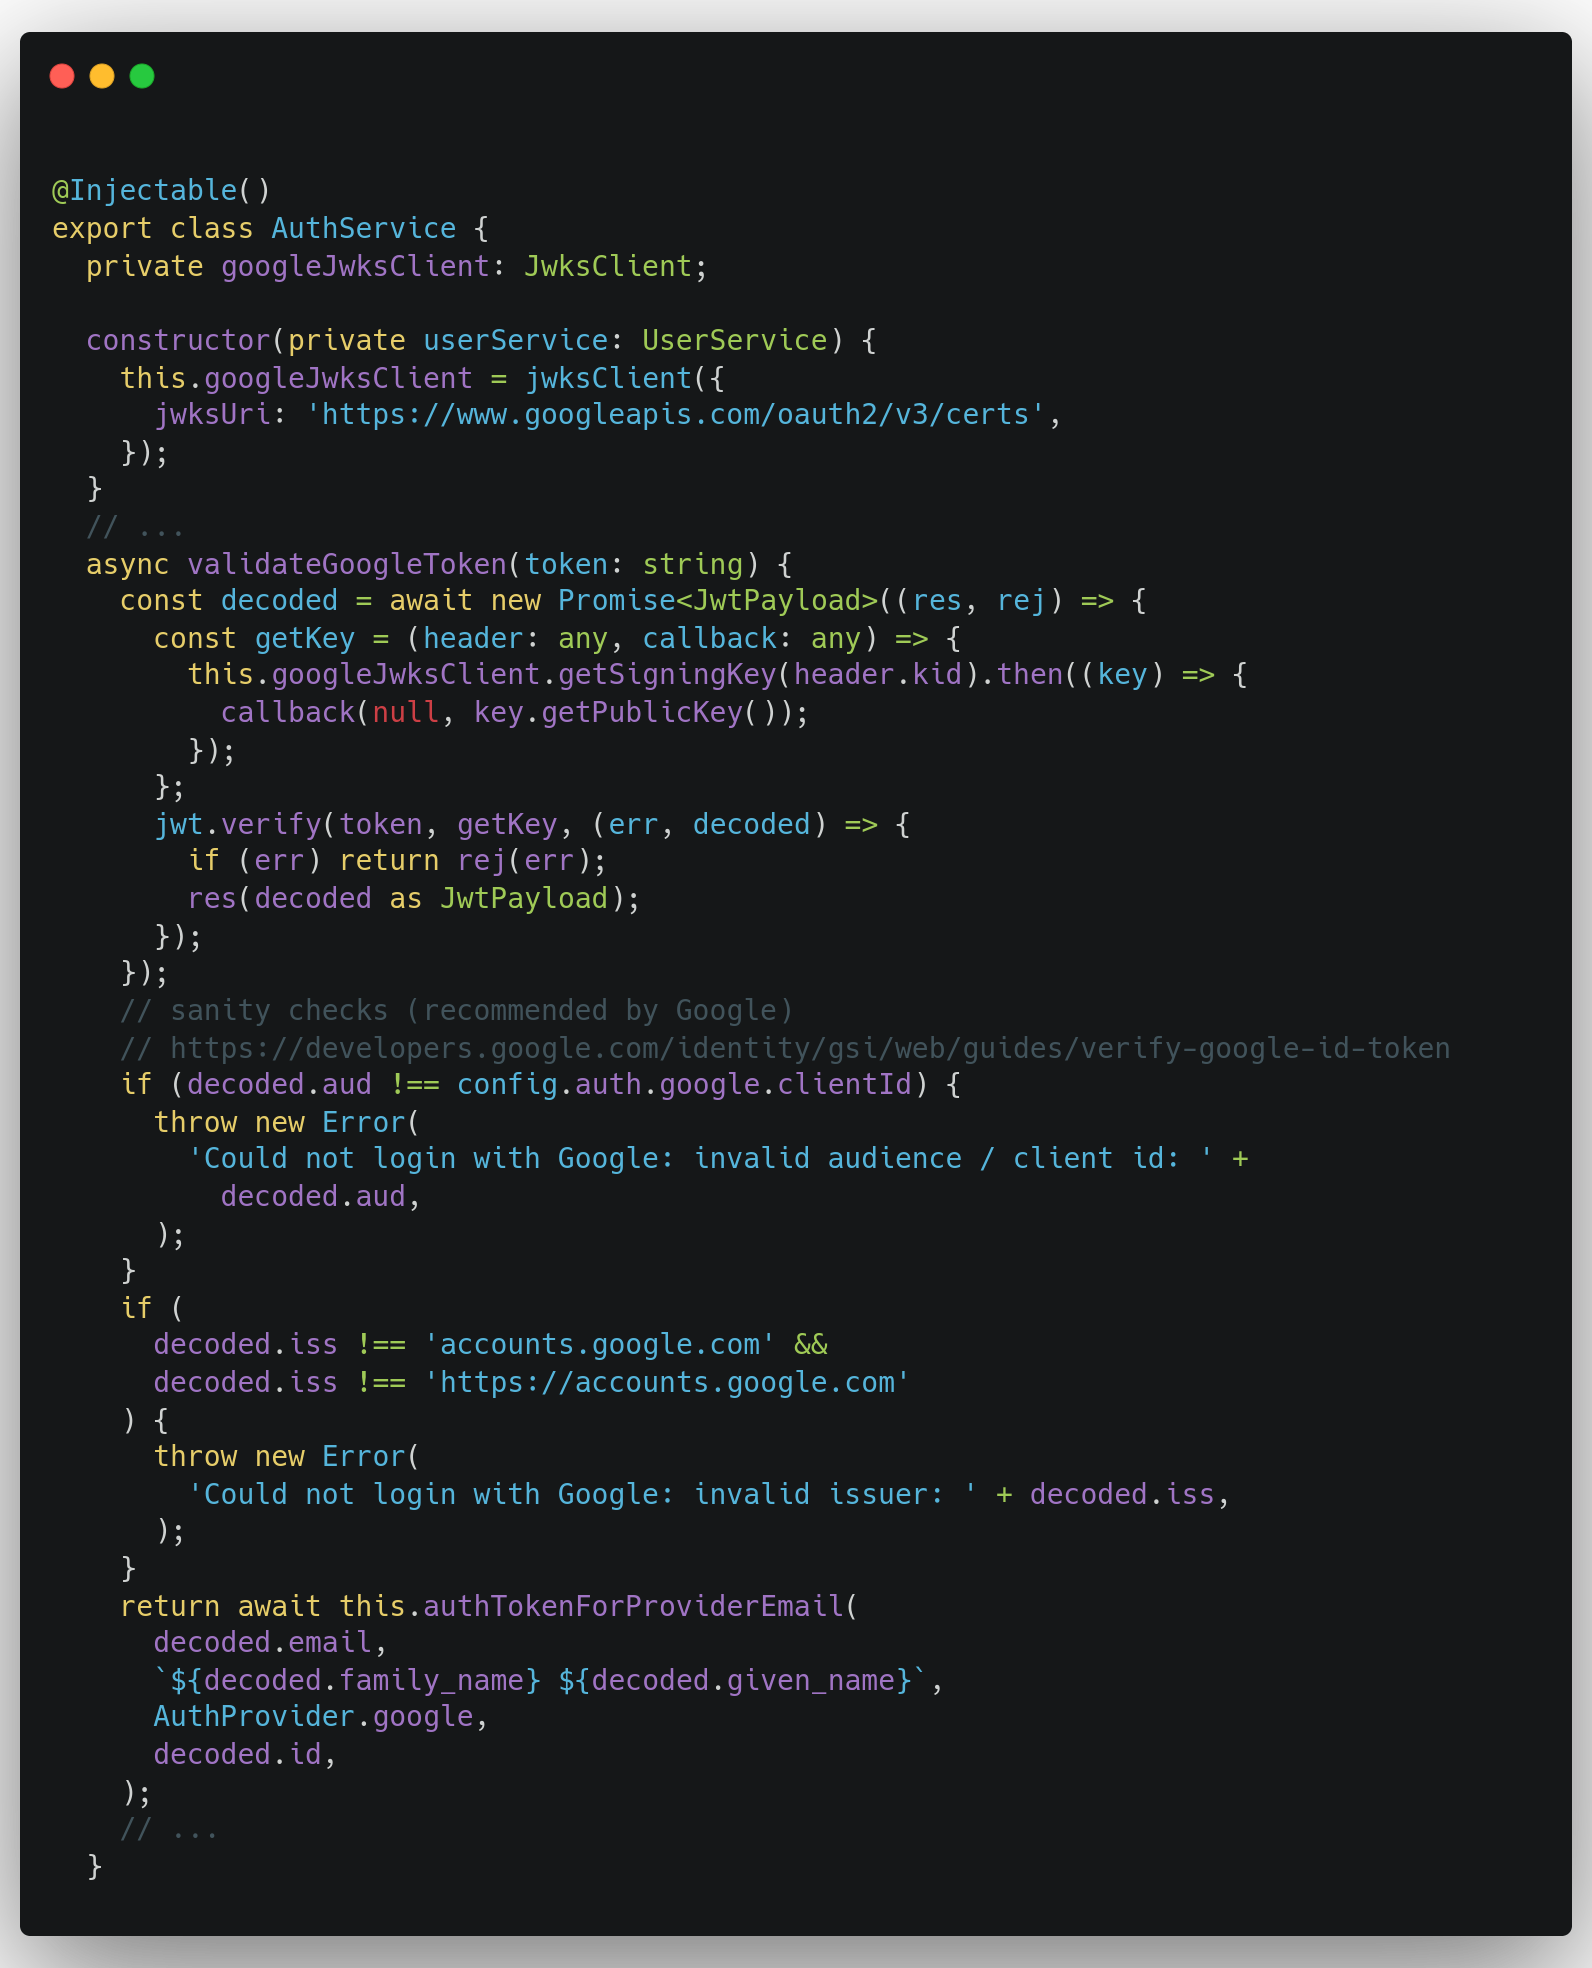
\includegraphics[width=0.9\textwidth]{./figures/code/be_auth-service-google.png}
    \caption{Backend: code that validates Google JWT tokens, for Google sign-in.}
    \label{FigBeAuthServiceGoogle}
\end{figure}

The Auth module has functionality related to user authentication: validating social logins, validating username and passwords, generating JSON Web Tokens (JWTs) and validating those tokens.

Google Sign-in is validated using a token received from the frontend and emitted by Google. The token is a JWT that is encoded using a JSON Web Key (JWK). Google publishes the public keys they use in a JSON Web Key Set (JWKS) format, which can be used to validate JWT tokens emitted from them, and verify their authenticity. Google also recommends performing a set of sanity checks on the JWTs apart from checking their signature, to prevent various attacks, such as emitting valid JWTs for a different application, or from a different Google service. The JWT signature verification library used in the app also makes sure that \verb|iat| and \verb|exp| are enforced (disallowing expired tokens). See Figure \ref{FigBeAuthServiceGoogle} for a code snippet of this step.

Yahoo Sign-in is validated by redirecting the user through a traditional OAuth authorization flow. At the end of the frontend flow, the backend receives a code that will then be sent to Yahoo (using a REST API) for validation, resulting in an \verb|access_token| that grants permission to Yahoo's OAuth APIs. The backend then makes a request to the userinfo endpoint, retrieving the user's email.

Upon validating social credentials, the backend then checks for an user account that already exists in the database (matching using the user's email as received from the social provider), creating one if one doesn't already exist. For this user id, a JWT token is emitted using the application secret (as defined in the configuration, see Section \ref{sec:Configuration}), and returned to the frontend.

The \verb|AuthModule| also provides methods to verify user JWTs, and a Request Guard that can be used to guard API routes that require authentication. Validating JWTs from API requests is done via a library called \verb|passport| and its Nest integration \verb|@nestjs/passport|. Making use of the JWT passport strategy, we can easily configure a strategy that checks JWTs received in the \verb|Authorization| header, via the application's JWT secret. The code is available in Figure \ref{FigBeJwtStrategy}, where it can be noticed how we configure \verb|passport| to validate JWTs, and tell it how to retrieve a user from a valid JWT by making use of the \verb|AuthService|.

\begin{figure}[htbp]
    \centering
    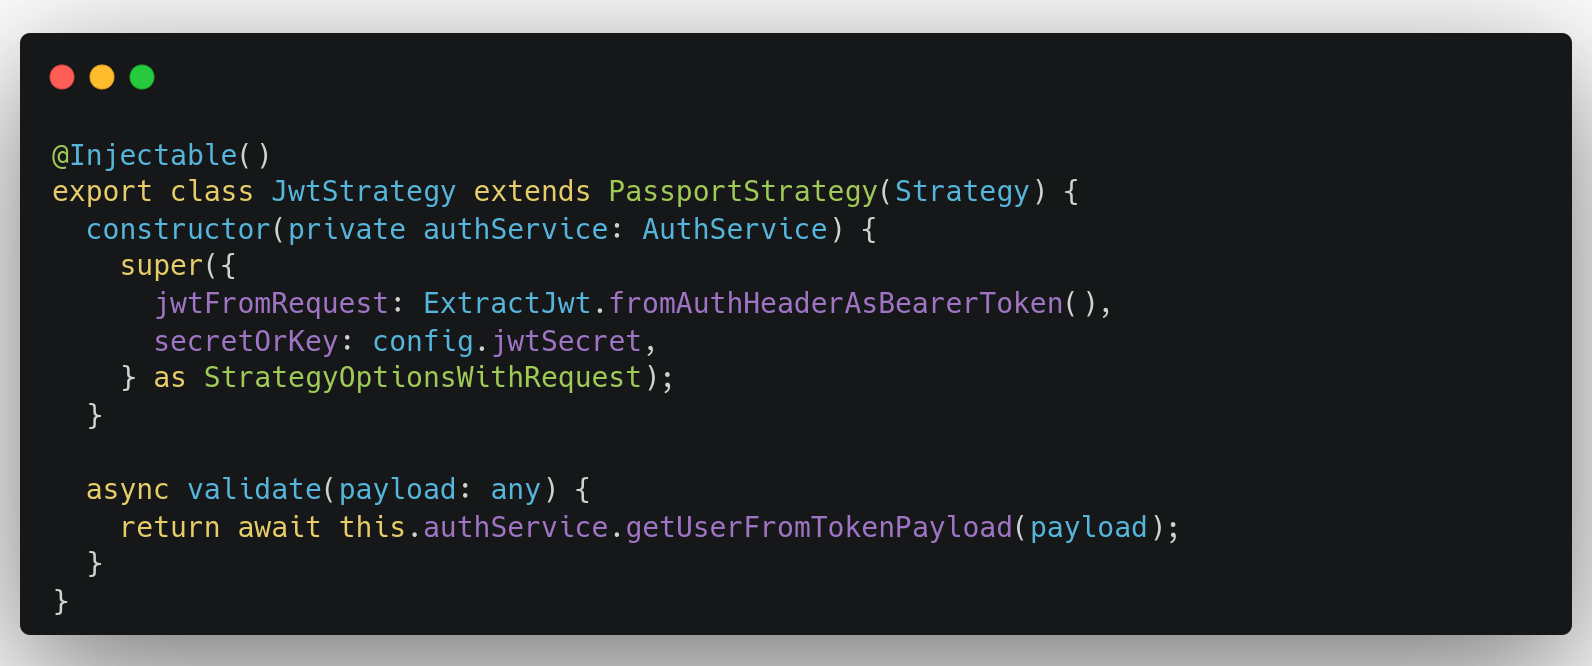
\includegraphics[width=1\textwidth]{./figures/code/be_jwt-strategy.png}
    \caption{Backend: the JWT strategy, as defined using @nestjs/passport.}
    \label{FigBeJwtStrategy}
\end{figure}

A popular method of accessing user data pertaining to a request, in the Express framework, is by attaching a \verb|user| property on the \verb|req| (Request) object. This object is passed around to all handler code in the app, making it an easy way of passing request state around the application. Nest abstracts away this \verb|req| object, and although it provides ways of accessing it, they are discouraged in lieu of a more opinionated approach, that is less prone to type errors. The Nest approach of decoding the user from the request consists of creating a decorator that makes this decoding for us, and places the user object into a parameter of choice in the controller code. The definition of this decorator, along with an example, is shown in Figure \ref{FigBeReqUser}.

\begin{figure}[htbp]
    \centering
    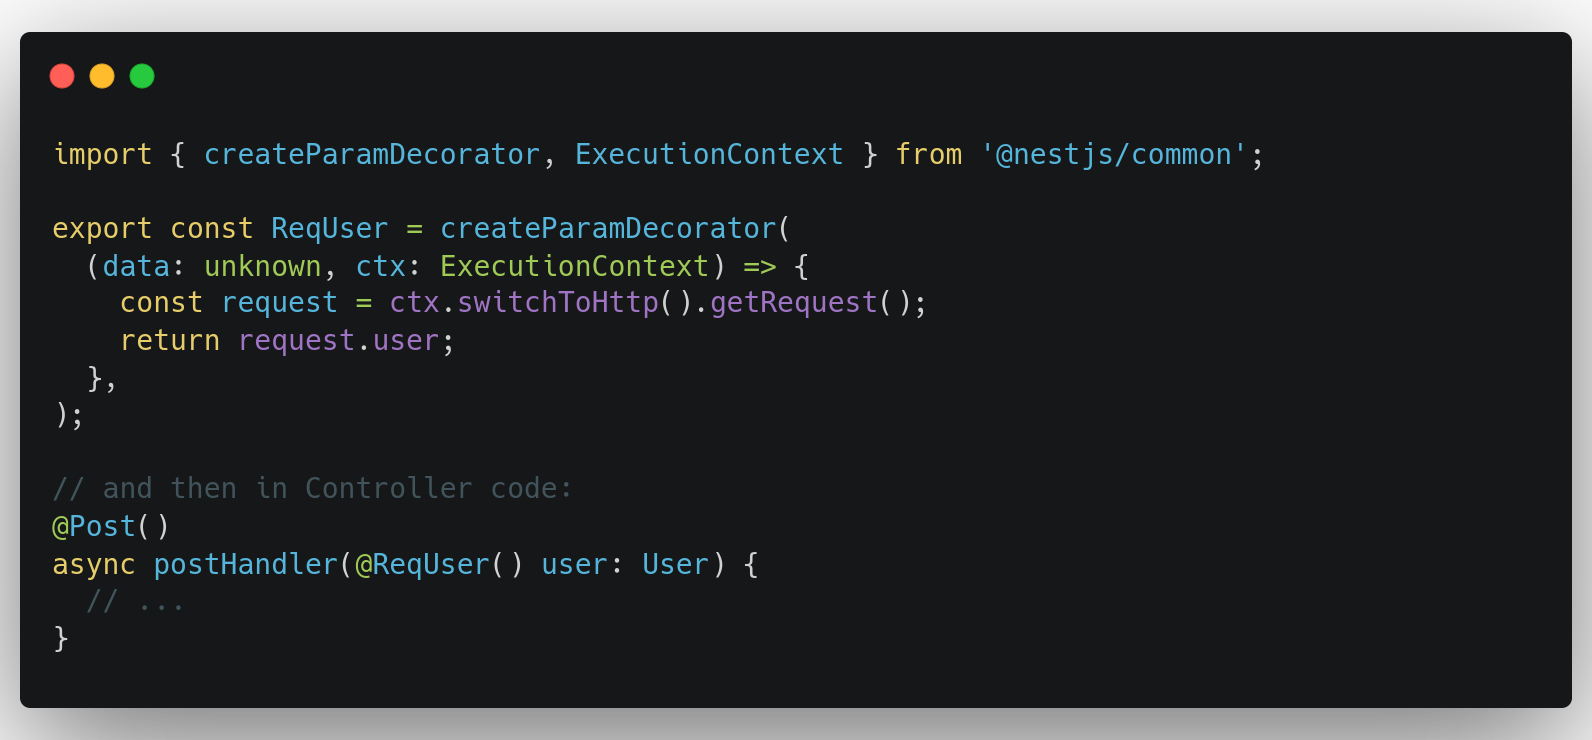
\includegraphics[width=1\textwidth]{./figures/code/be_req-user.png}
    \caption{Backend: the definition of the @ReqUser() decorator, along with an usage example.}
    \label{FigBeReqUser}
\end{figure}

\subsection{DTO validation}

All request validation throughout the app is performed using Data Transfer Objects (DTOs), that are annotated with specific validation criteria.